\documentclass{article}
\usepackage[utf8]{inputenc}
\usepackage[T1]{fontenc}
\usepackage{graphicx}
\usepackage{hyperref}
\usepackage{geometry}
\geometry{margin=1in}

\title{Britannica Volume 144850379 Row 1942}
\date{Encyclopaedia Britannica (1771)}

\begin{document}
\maketitle

\section*{Historical source}
\textbf{Entry ID:} \texttt{entry-britannica-volume-144850379-row-1942-1942} \\
\textbf{Volume ID:} 144850379 \\
\textbf{Character Count:} 6060

\subsection*{Extracted Text}
PHAR MACY.

Prepara-
tions.

brought from Italy, are prepared in this manner. The
odorous parts may be again separated from the oil,
and transferred into water or fpirit, by distillation with
those liquors.

Sect: IV. \_Conferration of recent Vegetables and\_
\_their Infusions, etc. by Sugar and Honey.\_

§ 1. CONSERVES.

454. CONSERVES are compollions of recent vege
table matters and fugar beaten together into an uni-
form mafs.

This management was introduced for preferving
certain samples, undried, in an agreeable form, with
as little attention to poblin in their native viruses;
and to fome subjects it is very advantageously applied.
Vegetables, whole virus use all or delivered in dry-
ing, except in this form be kept unjusted for a length
of time; For, by carefully focusing the mouth of the
containing wells, the alteration, as well as diffusion,
of their either principles, is generally prevented, and
the fugar preserves them from the corruption which
joley vegetable would otherwise undergo.

There are, however, fundry vegetables whole vi-
tous are impaired by this treatment. Muchaginous
fubilances, by long lying with fugar, become leis glu-
tionus, and that甚antly fully follow them the pa-
late. Many of the fingers flowers are of to tender
and delicate a texture, as almost entirely to lode their
peculiar qualities on being been on brushed
in general. It is obvious, that in this form, on ac-
count of the large admixture of fugar, only fulbliances
of considerable activity can be taken to advantage as
medicines. And indeed, conferve are at perfect con-
fidered chiefly as auxiliaries to medicines of greater
efficacy, as interventions for joining them together.
They are very convenient for echoing into boubles or
pills the more pondrous powders, as mecurunu dul-
cies, the colors of iron, and other mineral preparations;
which will liquid or leis confident matters, as fyrroup,
will not cohere.

The flops were formerly ecumulated with many
conferences altogether insignificant; the few now retain-
ed have in general either an agreeable flavour to re-
commend them, or are capable of answering some
ofeful purpose as medicine. Their common dole is
the bulk of a nutmey, or as much as can be taken up
at once or twice upon the point of a knife. There is
in general no great danger of exceeding in this parti-
cular.

455. \_General method of preferring conferences\_.

Leaves are picked from the flalks, and flowers from
their crops. They are beaten in a marble mortar,
with a wooden peille, into a smooth mafs after
which three there weight of double-refined fugar is
added by degrees, and the beating continued till
they are uniformly mixed.

The fugar should be pulverified by infilt, and patfed
through a fleeve, before it is mixed with the vegetable
mafs; otherwise it cannot easily be reduced to folfix-
cleine friends, fo as to be daily incorporated. Some
vegetables are cause reducible to the requisite finerals
by beating in a mortar; fuch is orange-peel. This
is molt conveniently raffed or grated off from the
finis, then well mixed with the fugar, and the com-

Part II.

pound fet by in a clole veffel for fome weeks; after
which it may be beaten Smooth with confidierably leis
labour than at frift. This peel, and red role-buds,
are commonly ground in a wooden mill made for that
purpole.

456. \_Conferve of the leaves of garden fuancy-grafs\_. L.

This is the only form that feury-grafs in futultance
can be kept in without the total line of its virtues.
The conferve retains the full suite and virtue of the
herb for a very conferable length of time, as a year
two, provided the veffel be made perfectly cleo
and ice in a cool place. It must be given in Ecurbotic
habits three or four times a-day, so efficient.

437. \_Conferve of the leaves of wood-forrel\_. L.

This is a very elegant and grateful conferve y in
talte it is lightly cushion, with a peculiar flavory
which home refranchise totals of green-taa. It is taken
because for quenching thirk, and cooling the
mouth and fauces, in hot distempers. It may be uife-
fully joined to the foregoing preparation, whole vic-
ture to fomelan promotes, at the same time that it
improves the taille.

458. \_Conferve of the leaves of jewarmist\_.

The conferve of mini retains the safe and virtues
of the herb. It is given in weakouts of the stomach
and perhaps to omit; and not unfrequently deea
fervice in fome cafes of this kind, where the warmer
and more active preparations of mini would be leis
proper.

459. \_Conferve of the leaves of rugs\_. L.

This conferve is given from a dram to half an ounce
in crudities of the prime via, for promoting digestion,
and in by their disorders; I gently illuminate the fo-
lids, attenuates vital juices, and excites the natural
feecretions. Some have had a great opinion of it, ta-
ken in a morning, as a preferative against the effects
of contagious air or calitation.

460. \_Conferve of the tops of jau-mesorwood\_. L.

The conferve of wormwood has been celebrated in
droplets. Mathihulus relates, that several persons were
cured by it of that diltemper, without the diffiance
of any other medicine. Where the diforder indeed
proceeds from a simple laxity or flagidity of the fo-
lids, the contained use of this medicine may be of bone
ferives, as it appears to be a not malignant mild cor-
robranant. It is directed to be given in the dole of
half an ounce, about three hours before meals.

461. \_Conferve of the buds of red refer\_.

This is a very apparent and useful concre. A
dram or two, diluted in warm milk, are frequently
given as a light refrigerant in weakness of the blo-
month, and likewise in couple and phithical com-
plaints. In the German Ephemerides, examples are
related of very dangerous phihifies cured by the con-
tinned out of this medicine; in one of the cafes, zo
pounds of the conferve were taken in the face of a
month; and in another, upwards of go. Riverius
mentions federal other influences of this kind.

461. \_Conferve of refractory-flowers\_. L.

Rofernary-flowers in great incature loft their pecu-
liar



\section*{Source record}
\begin{itemize}
\item \textbf{Dataset:} \texttt{NationalLibraryOfScotland/encyclopaedia\_britannica\_illustrated}
\item \textbf{Dataset Revision:} \texttt{309f765b1ecc83e0a7f7762e44b4a927a7555443}
\item \textbf{Page ID:} \texttt{britannica:309f765b1ecc83e0a7f7762e44b4a927a7555443:train:1942} \\
  \textbf{Filename:} \texttt{page-1942-99b5dc3b4c6c.jpg} \\
  \textbf{Row Index:} 1942 \\
  \textbf{SHA256:} \texttt{99b5dc3b4c6cd19e...}
\end{itemize}

\begin{figure}[h]
\centering
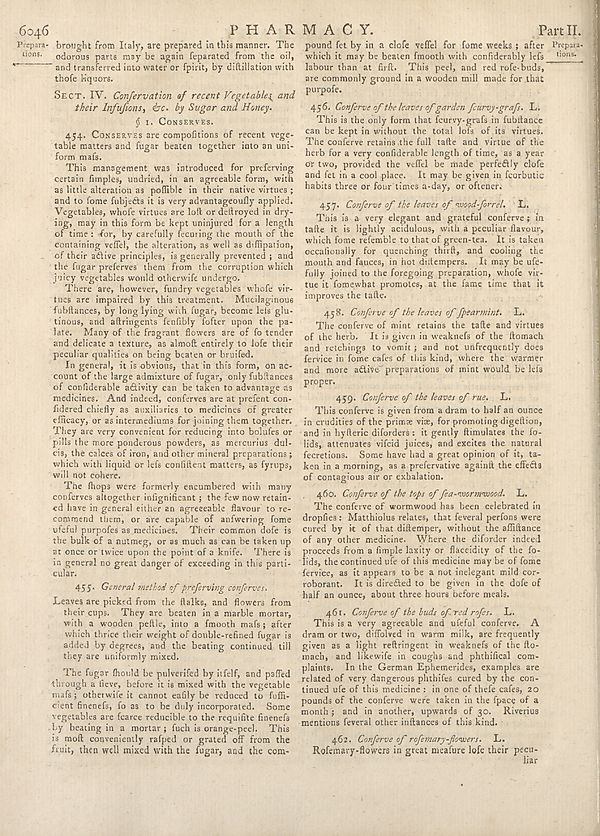
\includegraphics[width=0.85\textwidth]{../scans/page-1942-99b5dc3b4c6c.jpg}
\caption*{Source scan: \texttt{page-1942-99b5dc3b4c6c.jpg}}
\end{figure}

\end{document}
